
All used languages have functional and concurrent built-in features, with the first ones supporting the second ones. Erlang and Scala’s implementations are based in the actor pattern for doing parallel computation. Clojure on the other hand works with the agent concept, a similar model with simplified ways of reading the involved information.

To communicate modules we used language’s dependent (different) data types. The message's structure was tuples for Erlang and Scala, and for agents it was necessary to encapsulate functions on protocols (Clojure variants of Java interfaces). For sharing individuals (the pool) we used functionals consult/modification data structures: hash-like for Scala/Clojure and the {\em ets} module in Erlang’s case. The data was encoded with compound data structures: lists, vectors, tuples, records, etc. The Table \ref{tb:res:comp} summarizes the differences between the languages.

\begin{table}
  \caption{Language's comparisons.}\label{tb:res:comp}
  \centering
  \begin{tabular}{|p{4cm}|>{\centering}p{3cm}|>{\centering}p{3cm}|>{\centering}p{3cm}|}
    \hline
     & \textbf{Erlang} & \textbf{Scala} & \textbf{Clojure} \tabularnewline
    \hline
    Parallel executing unit & actor & actor & agent \tabularnewline
    \hline
    Communication (messages) & tuple & tuple & function (protocol) \tabularnewline
    \hline
    pool & \texttt{ets} & HashMap & hash-map \tabularnewline
    \hline
    DS chromosome & list & list & vector \tabularnewline
    \hline
    DS population & list & list & lazy list \tabularnewline
    \hline
    Compound data & tuple & tuple/object & record/vector \tabularnewline
    \hline
    Runtime environment & Erlang VM & Java VM & Java VM \tabularnewline
    \hline
  \end{tabular}

\end{table}


\simpleEntry{Results}

The design was tested with a population of 1024 individuals on each
island (two islands were used), doing 5000 evaluations on a dual-core
laptop  i7 with Windows 8 and 16 Gb of RAM. In order to find the
betters combinations of evaluators/reproducers was tested several of
them for each technology (evaluators = $1..30$ and reproducers =
$1..10$), in all the combinations the number of evaluators is greater
than the reproducers because the fitness function is more
computational intensive than the reproduction execution. It was used
10 runs for each combinations and later was deleted the times with
more dispersion until the standard deviation (SD) remains below the 5
\%. 

For a speedup analysis, using the ideas presented in \cite{Alba02parallelevolutionary}, it was made a sequential implementation with the same data structures and operator's implementations. Speedup is the ratio between $E[T_1]$ (sequential implementation average time) and $E[T_m]$ (parallel implementation average time in $m$ processors), the expected value is $m=4$ in this case (the number of logical processors in the hardware used).

\begin{table}
  \caption{Experiment results for the minimum parallel time of all combinations tested (time in milliseconds).}\label{tb:resAll}
  \centering
\begin{tabular}{|>{\centering}p{1.6cm}|>{\centering}p{2.5cm}|
>{\centering}p{2.4cm}|>{\centering}p{2.1cm}|>{\centering}p{1.7cm}|
>{\centering}p{1.45cm}|>{\centering}p{1.45cm}|}
  \hline
  \textbf{Language} & \textbf{Parallel time $\pm$ SD} & \textbf{Workers combination} & \textbf{Sequential time} & \textbf{Relative speedup} & \textbf{Speedup}\tabularnewline
  \hline
  Erlang & 2920.40 $\pm$ 126 & 25 evaluators, 1 reproducer & 8143.3 & 2.7884 & 0.5519 \tabularnewline
  \hline
  Clojure & 1734.66 $\pm$ 28.32 & 10 evaluators, 1 reproducer & 3340.2222 & 1.9255 & 0.9292 \tabularnewline
  \hline
  Scala & 563 $\pm$ 24.32 & 6 evaluators, 1 reproducer & 1651.8 & 2.8632 & 2.8632 \tabularnewline
  \hline
\end{tabular}
\end{table}

The results showed in Table \ref{tb:resAll} indicate for each language the best time for the parallel implementation, the combination of evaluators/reproducers in which the parallel variant was obtain, the time for the sequential implementation, a relative speedup (calculated in relation to his sequential time) and the speedup (relative to the best sequential time, Scala's in this case). Each worker (evaluators and reproducers) is an unit of execution and in the hardware used only 4 units (at most) can run at the same time.

\begin{figure}
\label{fig:oneRep}
\caption{Parallel running times for one reproducer.}
\centering

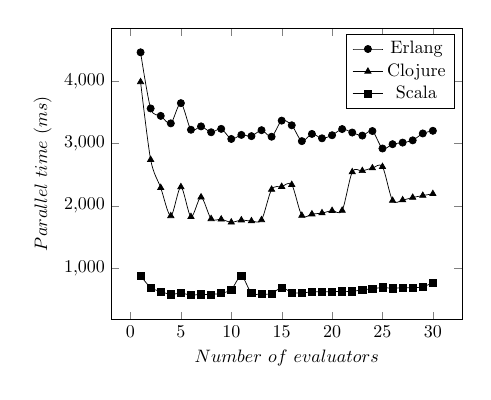
\begin{tikzpicture}[thick, scale=0.65]

  \begin{axis}[
         xlabel=$Number \hspace{.12cm} of \hspace{.12cm} evaluators$,
         ylabel=$Parallel \hspace{.12cm} time \hspace{.12cm} (ms)$
         ]
     \addplot[smooth,mark=*]  plot coordinates{
(1,4466.6)
(2,3564.222222222222)
(3,3444.6666666666665)
(4,3324.5555555555557)
(5,3649.6)
(6,3221.7)
(7,3275.9)
(8,3181.3)
(9,3236.0)
(10,3073.5555555555557)
(11,3139.0)
(12,3119.1111111111113)
(13,3214.9)
(14,3109.5555555555557)
(15,3368.3)
(16,3293.7)
(17,3039.1)
(18,3154.7)
(19,3084.1)
(20,3133.6666666666665)
(21,3232.9)
(22,3177.1111111111113)
(23,3128.0)
(24,3201.3333333333335)
(25,2920.4)
(26,2989.5555555555557)
(27,3015.4)
(28,3051.4444444444443)
(29,3162.3)
(30,3204.7)
     };
     \addlegendentry{Erlang}

     \addplot[smooth,mark=triangle*]
         plot coordinates{
(1,3990.75)
(2,2740.777777777778)
(3,2289.1111111111113)
(4,1837.111111111111)
(5,2302.5555555555557)
(6,1822.6666666666667)
(7,2138.6666666666665)
(8,1789.5)
(9,1782.3333333333333)
(10,1734.6666666666667)
(11,1768.888888888889)
(12,1754.7777777777778)
(13,1772.0)
(14,2261.1111111111113)
(15,2307.8888888888887)
(16,2338.4444444444443)
(17,1842.3333333333333)
(18,1865.7777777777778)
(19,1883.4444444444443)
(20,1920.7777777777778)
(21,1923.5)
(22,2542.1111111111113)
(23,2561.6666666666665)
(24,2605.5555555555557)
(25,2627.0)
(26,2083.0)
(27,2091.8888888888887)
(28,2132.222222222222)
(29,2163.777777777778)
(30,2192.1111111111113)
         };
     \addlegendentry{Clojure}


     \addplot[smooth,mark=square*]
         plot coordinates{
(1,876.6666666666666)
(2,683.7777777777778)
(3,622.2857142857143)
(4,575.2222222222222)
(5,596.0)
(6,563.0)
(7,576.2222222222222)
(8,574.0)
(9,595.1111111111111)
(10,651.8888888888889)
(11,871.6666666666666)
(12,595.3333333333334)
(13,582.25)
(14,586.8888888888889)
(15,684.8888888888889)
(16,605.0)
(17,600.625)
(18,614.0)
(19,618.2222222222222)
(20,616.7777777777778)
(21,625.2222222222222)
(22,622.6666666666666)
(23,649.7777777777778)
(24,664.1111111111111)
(25,686.625)
(26,672.4444444444445)
(27,684.7777777777778)
(28,681.625)
(29,698.0)
(30,760.7142857142857)
         };
     \addlegendentry{Scala}

  \end{axis}

\end{tikzpicture}


\end{figure}

\begin{figure}
\label{fig:twoRep}
\caption{Parallel running times for two reproducers.}
\centering

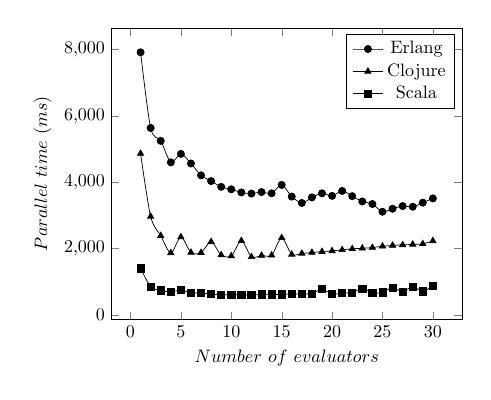
\begin{tikzpicture}[thick, scale=0.65]

  \begin{axis}[
         xlabel=$Number \hspace{.12cm} of \hspace{.12cm} evaluators$,
         ylabel=$Parallel \hspace{.12cm} time \hspace{.12cm} (ms)$
         ]
     \addplot[smooth,mark=*]  plot coordinates{
(1,7919.428571428572)
(2,5638.0)
(3,5249.75)
(4,4601.5)
(5,4856.714285714285)
(6,4567.285714285715)
(7,4208.333333333333)
(8,4036.0)
(9,3862.777777777778)
(10,3788.3)
(11,3693.6)
(12,3659.2)
(13,3705.1111111111113)
(14,3667.0)
(15,3920.4)
(16,3568.2)
(17,3376.75)
(18,3544.7)
(19,3668.222222222222)
(20,3589.4)
(21,3739.222222222222)
(22,3580.9)
(23,3421.6)
(24,3345.222222222222)
(25,3110.8)
(26,3202.4)
(27,3282.1)
(28,3262.0)
(29,3385.4)
(30,3513.777777777778)
     };
     \addlegendentry{Erlang}

     \addplot[smooth,mark=triangle*]
         plot coordinates{
         (1,4866.5)
(2,2970.0)
(3,2389.5555555555557)
(4,1870.5555555555557)
(5,2347.1111111111113)
(6,1882.888888888889)
(7,1878.111111111111)
(8,2206.1111111111113)
(9,1808.4444444444443)
(10,1777.3333333333333)
(11,2238.1111111111113)
(12,1752.3333333333333)
(13,1791.888888888889)
(14,1798.888888888889)
(15,2324.777777777778)
(16,1825.7777777777778)
(17,1854.5555555555557)
(18,1881.5555555555557)
(19,1908.6666666666667)
(20,1931.5555555555557)
(21,1962.888888888889)
(22,1993.6666666666667)
(23,2010.111111111111)
(24,2030.5555555555557)
(25,2071.0)
(26,2094.3333333333335)
(27,2112.8888888888887)
(28,2126.4444444444443)
(29,2144.5555555555557)
(30,2233.222222222222)
         };
     \addlegendentry{Clojure}


     \addplot[smooth,mark=square*]
         plot coordinates{
(1,1406.8333333333333)
(2,854.5714285714286)
(3,741.0)
(4,694.75)
(5,752.2)
(6,660.1111111111111)
(7,663.4285714285714)
(8,626.5)
(9,605.375)
(10,609.125)
(11,602.7777777777778)
(12,596.1428571428571)
(13,620.8888888888889)
(14,619.7777777777778)
(15,619.0)
(16,634.2222222222222)
(17,631.8888888888889)
(18,641.8888888888889)
(19,775.5555555555555)
(20,630.625)
(21,656.6666666666666)
(22,672.7777777777778)
(23,796.2222222222222)
(24,671.1111111111111)
(25,679.3333333333334)
(26,825.8888888888889)
(27,696.2222222222222)
(28,854.5)
(29,711.0)
(30,882.6666666666666)
         };
     \addlegendentry{Scala}

  \end{axis}

\end{tikzpicture}


\end{figure}

The Figure 1 shows the running times when one reproducer was used with a variant number of evaluators and Figure 2 shows the same for tow reproducers. In the tow cases the overall behaviour of Scala is the best. Due to that computation complexity of the evaluation function is greater than the reproduction phase the results when one reproducer was used are better than when tow reproducers was used.

Scala implementation are smoother in his results in contrast with Clojure's in which many peaks was obtained. This tow languages use the JVM and the same random library, therefor there is a clear differences in theirs concurrent models. The results in Scala and Clojure was better with small number of units of execution: when the number of evaluators grows the efficiency of the algorithm falls. In this matter Erlang had a non-typical behaviour and it was improving until 25 evaluators, only then the speed began to decrease.

Erlang was the language with the worst execution time; but it's runtime, in the best case, was able to schedule 52 units of execution (far more than the others). Also the speedup obtained relative to his sequential time are very good, this two facts point to a possible good scalability. Clojure's performance is medium, with a speedup close to $1$.

Scala was the language with the best results, even when it's runtime are the same of Clojure's, his models of computation and concurrency (in particular his balance between mutable and immutable state) allow a better behaviour of the concurrent algorithms. Again is important to note the quality of the concurrent abstractions made by all this technologies in which the number of logical units of executions are greater than the number of the physical ones.
